\documentclass[aip]{revtex4-1}
\usepackage{graphicx}
\usepackage{color}
\usepackage{hyperref}
\usepackage{braket}
\usepackage{mhchem}
\begin{document}
\title{Supplementary Information:
Improving the efficiency of $G_0W_0$ calculations with approximate spectral decompositions of dielectric matrices: Supplementary information}
\renewcommand{\figureautorefname}{Fig.}

\author{Han Yang}
\affiliation{Department of Chemistry, University of Chicago, Chicago, Illinois 60637, United States}
\affiliation{Pritzker School of Molecular Engineering, University of Chicago, Chicago, Illinois 60637, United States}

\author{Marco Govoni}
\affiliation{Pritzker School of Molecular Engineering, University of Chicago, Chicago, Illinois 60637, United States}
\affiliation{Materials Science Division and Center for Molecular Engineering, Argonne National Laboratory, Lemont, Illinois 60439, United States}


\author{Giulia Galli}
\email[]{gagalli@uchicago.edu}
\affiliation{Department of Chemistry, University of Chicago, Chicago, Illinois 60637, United States}
\affiliation{Pritzker School of Molecular Engineering, University of Chicago, Chicago, Illinois 60637, United States}
\affiliation{Materials Science Division and Center for Molecular Engineering, Argonne National Laboratory, Lemont, Illinois 60439, United States}

\date{\today}

\maketitle

This Supplementary Information reports convergence studies of the G$_0$W$_0$ calculations of the vertical ionization potential of the CH$_4$ molecule, whcih is taken as a representative example of the molecular systems studied in the main text.

\section*{$G_0W_0$ calculations of the vertical ionization potential of the methane molecule}
\subsection{Eigenvalues of the symmetrized \textit{irreducible} density-density response function}
In \autoref{fig:compare_eigenvals}, we  compare eigenvalues for the symmetrized irreducible density-density response function of the methane molecule: 500 stdPDEPs and 100 stdPDEPs +  400 kinPDEPs. On the scale of the figure the results are indistinguishable.

\subsection{Calculations of the vertical ionization potential}
We present, in \autoref{fig:different_number_of_PDEPs}, the results for the vertical ionization potential of the $\mathrm{CH_4}$ molecule computed with 5, 10, 20 standard PDEPs ($N_\mathrm{stdPDEP}$), and the remaining 100, 200, 300 and 400 PDEPs treated as kinetic PDEPs. When setting $N_\mathrm{stdPDEP}$ = 10 or 20 we obtain results accurate within 0.02 eV, as compared to the ones obtained using only standard PDEP. When using 5 stdPDEPs we obtain instead an error more than 10 times larger (0.25 eV).

\subsection{Interpolation of results}
In this work, the computed energy levels  were  interpolated with respect to the total number of PDEPs,
\begin{equation}
    E = a + \frac{b}{N_\mathrm{stdPDEP}+N_\mathrm{kinPDEP}},
\end{equation}
where $a$ is the converged energy level and $b$ is an arbitrary number depending on the system.

In \autoref{fig:interpolation_from20}, we show results for the vertical ionization potential  of the methane molecule with respect to the total number of PDEPs included in the calculation: 20 stdPDEPs were used followed by 0, 100, 200, 300, 400 kinPDEPs. We note that as the number of  kinPDEPs increases, one obtains energies similar to those computed with stdPDEPs; in addition the proportionality between energies and the inverse of the total number of PDEPs holds even when the total number of PDEPs in small.


\begin{figure}
    \centering
    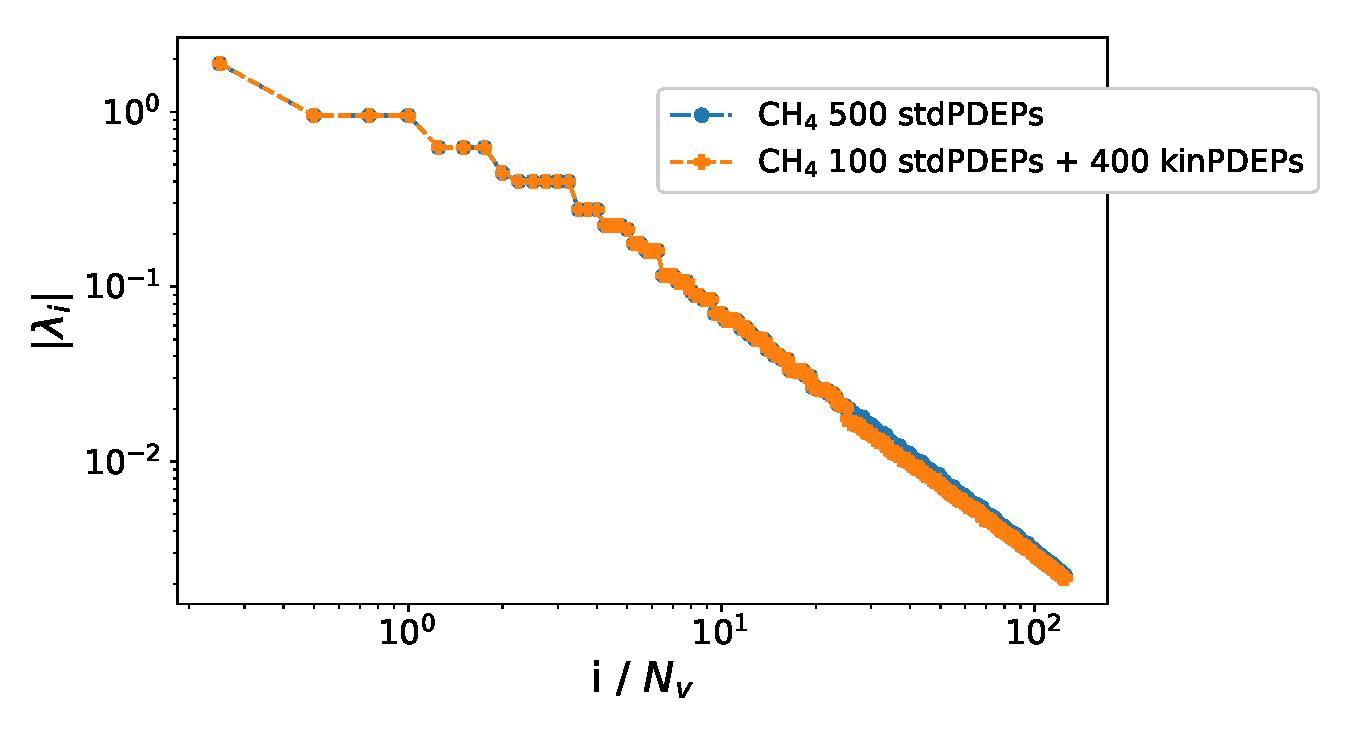
\includegraphics[width=0.8\linewidth]{fig/Compare_PDEP_eigenvals_and_mix_eigenvals.eps}
    \caption{Comparison between the eigenvalues ($\lambda_i$) of the leading 500 stdPDEPs and the eigenvalues of the 100 leading stdPDEPs followed by 400 kinPDEPs of the CH4 molecule. $N_v$ is the number of occupied states and stdPDEPs and kinPDEPs are eigenvectors of the symmetrized irreducible density-density response function($\tilde{\chi}_0$) solved using Kohn-Sham Hamiltonian and kinetic operator.}
    \label{fig:compare_eigenvals}
\end{figure}

\begin{figure}
    \centering
    \includegraphics[width=0.8\linewidth]{fig/Fitting_from_different_stdPDEP.eps}
    \caption{Calculations of the vertical ionization potential of the methane molecule with 20, 10, 5 standard eigenpotentials (stdPDEP) and up to 400 kinetic eigenpotentials (kinPDEP) compared to calculations (red symbols) performed  with purely stdPDEPs.}
    \label{fig:different_number_of_PDEPs}
\end{figure}

\begin{figure}
    \centering
    \includegraphics[width=0.8\linewidth]{fig/Fitting_example_of_CH4_1_to_N.eps}
    \caption{Interpolation of the computed vertical ionization potential of the methane molecule with respect to the total number of PDEPs, where PDEPs are eigenvectors of the symmetrized irreducible density-density response function ($\tilde{\chi}_0$).}
    \label{fig:interpolation_from20}
\end{figure}

\end{document}